\documentclass[12pt]{article} 
\usepackage[pdftex]{graphicx}
\usepackage{natbib} 
\usepackage{color}
\usepackage{amsmath} 
\usepackage{amssymb} 
\usepackage{verbatim}
\usepackage{mathpazo} 
\usepackage{setspace}
\usepackage{multirow}
\usepackage{fullpage}
\usepackage{lscape}
\usepackage{fancyhdr}
\usepackage[normalem]{ulem} 
\usepackage{hyperref}
\usepackage[parfill]{parskip}
\usepackage{xr}
\usepackage{paralist}
\usepackage{xr}
\externaldocument{SI}
\hypersetup{colorlinks=true, linkcolor=black, citecolor=black}
\RequirePackage{lineno}

\newcommand{\flagged}[1] {
  \textcolor{blue}{#1}
}

\def\title{The temporal assembly of plant-pollinator networks
  following restoration}
\def\author{Lauren C.\ Ponisio$^{1,2}$, Marilia P. Gaiarsa$^3$, Claire
  Kremen$^1$}

\def\runninghead{Plant-pollinator network assembly}
\def\keywords{community assembly, change points, specialization,
  nestedness, modularity, bipartite, preferential attachment}

\def\extras{
  \begin{itemize}
  \item Submitted as a Letter
  \item Abstract word count: 
  \item Main text word count: 
  \item Number of references: 
  \item Number of figures:
  \end{itemize}
}

\def\affiliation{
  \begin{enumerate}
  \item Department of Environmental Science, Policy, and Management\\
    University of California, Berkeley\\
    130 Mulford Hall\\
    Berkeley, California, USA\\
    94720\\
  \item Department of Entomology\\
    University of California, Riverside\\
    417 Entomology Bldg.\\
    Riverside, California, USA\\
    92521\\
  \item Departamento de Ecologia\\
    Universidade de Sao Paulo\\
    Sao Paulo, SP, Brazil\\
    05508-900\\
  \end{enumerate}
}

\newcommand{\mstitlepage}{
  \paragraph{Running head:} \textsc{\runninghead}
  % \parindent=0pt
  \begin{center}%
    {\LARGE \title \par}%
    \vskip 3em%
    {\large
      \lineskip .75em%
      \begin{tabular}[t]{c}%
        \author
      \end{tabular}\par}%
    \vskip 1.5em%
  \end{center}\par
  \affiliation
}
\clearpage

\begin{document}

\mstitlepage
\doublespacing
\linenumbers
\clearpage

\begin{abstract}
  TO BE RE-WRITTEN
  The structure of networks is related to ability of communities to
  maintain function in the face of species extinction. Understanding
  network structure and how it relates to network disassembly,
  therefore, is a priority for system-level conservation biology.  We
  explore the assembly of plant-pollinator communities on native plant
  restorations in the Central Valley of California. The assembling
  communities are paired with unrestored field margins (controls) and
  mature (non-assembling) hedgerows. We determine whether there are
  change points in the assembly of the communities where the network
  undergoes significant reorganization. We are also ask how are the
  individual species changing their interaction patterns? What does
  this mean for the topology/resilience of the network? We also
  attempted to adapt a financial model to mutualistic networks. Our
  biggest difficulty with this approach was to translate the price
  term to mutualistic systems. We explored a range of approaches, such
  as number of visits a species performs. However, it seems that
  financial systems cannot be easily translated to mutualistic
  systems. In addition, we used a Changing Point Detection Algorithm
  to assess weather the different communities went through a critical
  reorganization on their interaction patterns. We were able to
  identify some changing points in the communities, and also to
  explore some general patterns commonly used to describe ecological
  networks. For example, on the network level, networks become
  increasingly modular and less nested, whereas on the species level,
  species become more specialized, as resources become more reliable.
\end{abstract}

Keywords: changing points, temporal networks, hedgerows, species
interactions, preferential attachment

\clearpage

\section*{Introduction}
\label{sec:introduction}

Global change has created a severe biodiversity crisis
\citep{barnosky2011has}. As species are lost, so are their
interactions, causing further coextinction cascades
\citep{dunn2009sixth}.  Mutualistic systems are particualrly at risk.
Ecological restoration plays an increasingly important role in
recovering biodiversity (CITATIONS). Because the structure of
interaction networks is related to ability of communities to maintain
function in the face of species extinction \citep{Memmott2004}, a key
restoration aim is to facilitate assembly of robust networks. Little
is known, however, about how restoration influences the assembly of
interaction networks, or ecological network assembly more generally.

To date, only two field studies have examined how networks assemble
over time, often using space for time gradients. \cite{Olesen2008} was
investigated day-to-day, temporal assembly of a plant-pollinator
network within a season, taking advantage of the extreme seasonality
of pollinator communities in Greenland.  \cite{Olesen2008} found that
within a season, the network assembly was similar to preferential
attachment. New species tended to interact with already well-connected
species, likely because these species are either more abundant or more
temporally persistent.


The mostly widely explored mechanism of network assembly, preferential
attachment \citep{barabasi1999emergence}, predicts that a new species
is more likely to interact with species that are already
well-connected \citep[''the rich-get-richer''
principle,][]{barabasi1999emergence}.

\item Studying primary succession along a glacier foreland,
  \cite{albrecht2010plant} found a similar pattern where nestedness, a
  pattern of interactions where a generalist core interacts with both
  specialist and generalist species, increased as the community
  aged. % Studying ``managed succession'' of a clear-cut pine forest,
  % \cite{devoto2012understanding} found changes in network structure
  % were explained by a combination of age, tree density and variation
  % in tree diameter. 
\item Even non-successional temporal dynamics suggest a stable core of
  generalists persist despite high turnover of peripheral species
  \citep{fang2012relative, diaz2010changes, alarcon2008year}.
\item In contrast to the ordered network build-up described by
  preferential attachment, assembly may be punctuated by significant
  reorganizations of interactions. For example, as new species are
  added, resident species change their interaction partners to
  minimize competition, or become extinct. Such significant
  reorganizations of interactions, or changing points, have been
  observed in networks \citep{peel2014detecting}.
\end{itemize}

\section*{Materials \& Methods}
\label{sec:methods}

\subsection*{Study sites and collection methods}
\label{sec:study-sites}

We surveyed plant-pollinator interaction networks of assembling
hedgerows (N=5), as well as in two types of non-assembling communities
to serve as controls: unrestored, weedy field margins (N=XX) and
established hedgerows (greater than 10 years since planting,
N=XX). The sites were located in the Central Valley of California in
Yolo, Colusa and Solano Counties. This area is comprised of
intensively managed agriculture -- primarily monocultures of
conventional row crops, vineyards and orchards. Hedgerows we planted
along field margins where they do not remove valuable land from
production, and are ca. 3--6m wide and approximately 350m long and
border large (ca.\ 30--hectare) crop fields. Hedgerows consist of
native, perennial, shrub and tree plantings including \textit{Rosa
  californica}, \textit{Cercis occidentalis}, \textit{Ceanothus spp.},
\textit{Heteromeles arbutifolia}, \textit{Sambucus mexicana},
\textit{Eriogonum spp.}, \textit{Baccharis spp.}, \textit{Salvia
  spp}. and others \citep{kremen-2015-602, mgonigle-2015-x}. The mean
distance between monitoring sites was 15 km, and the minimum distance
between sites of the same type sampled in the same year was 2 km.  The
entire area surveyed spanned almost 300 km$^2$. The crop fields
adjacent to all sites were similarly managed as intensive, high-input
monoculture.

Monitoring began in 2006 and continued through 2015. Sampling of the
assembling hedgerows began the year before the area was restored. For
logistical reasons, no sampling of assembling hedgerows was conducted
in 2010. Sites were sampled between two and five times per year (Table
XX). In each round of sampling, the order in which sites were sampled
was randomized. Surveys were conducted under sunny conditions when the
temperature was above $21^{\circ}\mathrm{C}$ and wind speed was below
$2.5$ meters/second.

Flower-visitors to plants in hedgerows and unrestored controls were
netted for one hour of active search time (the timer was paused when
handling specimens). Honeybees (\textit{Apis mellifera}) were not
collected because their abundance is determined largely by the
placement of hives throughout the region by bee-keepers. All other
insect flower visitors that touched the reproductive parts of the
flower were collected; however, here we focus only on wild bees and
syrphids (representing XX and XX percent of records, respectively),
the most abundant and effective pollinators in the system (C. Kremen,
A. Klein and L. Morandin, unpublished data). Bee and syrphid specimens
were identified to species (or morpho-species for some bee specimens
in the genera \textit{Nomada} and \textit{Sphecodes}) by expert
taxonomists.

Quantitative networks were generative for each site through time. To
account for the unequal number of surveys between years, the mean of
the interactions between a pair of plants and pollinators across
surveys within a year was used as a representation of the frequency of
interactions.

\subsection*{Change point analysis}
\subsubsection*{Identifying change points}
We employed a change point detection method \citep{peel2014detecting}
to identify fundamental changes in large-scale pattern of interactions
of plants and pollinators. A change point is caused by a merge, split,
fragmentation or formation of communities (also called modules or
compartments). Change point detection methods have yet to be
generalized to quantitative networks, so for this analysis we focused
on qualitative (binary) networks. Following \cite{peel2014detecting},
we first defined a probability distribution over the networks using
the generalized hierarchical random graph model (GHRG). The GHRG model
is able to capture both assortative and disassortative community
structure patterns at all scales in the network
\citep{peel2014detecting}. A network $G$ is composed of vertices $V$
and edges $E \subseteq {V × V }$. The GHRG model decomposes the $N$
vertices into a series of nested groups, the relationships among which
are represented by the dendrogram $T$. The tips of $T$ are the
vertices of $G$, and the probability that two vertices $u$ and $v$
connect is given by the parameter $p_r$. The probability distribution
of the network $G$ thus defined as:

\begin{equation}
  \label{eq:lik}
  P(G|T,{pr}) = p_r^{E_r}(1-p_r)^{N_r-E_r}
\end{equation}
% 
Where $E_r$ is the observed number of edges between vertices with the
common ancestor $r$, and $N_r$ is the total possible edges.

Using Bayesian posterior inference and techniques from phylogenetic
tree reconstruction, we fit the GHRG model to the networks
\citep{peel2014detecting}. This is accomplished by using a Markov
Chain Monte Carlo (MCMC) procedure to first sample the posterior
distribution of bipartitions, from which a consensus tree is derived
\citep{peel2014detecting}. ADD NEWMAN PAPER. We used $\beta$
distributions with the hyperparameters $\alpha=\beta=1$ to define
priors for $p_r$.

Once the GHRG model has been fit to the networks, we determine whether
a change point occurred between two time slices. To detect a change
point, we compare the fit of two models -- one where a change point
had occurred between two networks, and one where no change occurred --
using posterior Bayes factors. We chose a sliding window of length,
$w$, of four, within which to find change points. Larger windows allow
for more gradual changes, and four was the maximum possible with our
maximum of nine years of data. Lastly, to calculate a $p$-value for
the Bayes factors, we use parametric bootstrapping to numerically
estimate the null distribution \citep{peel2014detecting}. The change
point analysis was carried out using code published online by L.~Peel.

We next test whether the change points occurring in maturing hedgerows
were a component of the assembly process or a product of environmental
shifts that lead to network reorganizations in all types of
communities. We model the number of change points as successes and the
total number of years each site was sampled as trails, and use a
generalized linear model with Binomial error to test whether the
probability of a change point occurring varied by site type. For the
non-assembling hedgerows and weedy field margins, only sites with five
or greater years of sampling was included in this analysis.

% \subsubsection*{Characteristics of species that contribute to change
%   points}

% To further elucidate the nature of the change points, we examine the
% characteristics of the species that contributed the reorganization of
% interactions. Some species remain in relativly similar network
% positions through time, whereas others are more variable in their role
% and thus contribute more strongly to network reorganization. If
% assembly is following according to a mechanism of preferential
% attachment, the more persistnet species with the higest degree would
% be most stable in their network position ???

% We test the hypothesis that the species that occupy the most stable
% positions in the network are the most temporally persistent and or
% generalized \citep{fang2012relative}.

% We calculate species persistence as the proportion of the surveys a
% pollinator was observed. Species observed consistently within and
% between years are thus maximally persistent. Species degree is based
% on plant-pollinator interaction observations from a more extensive
% data-set from Yolo County (approx.~ 18000 interaction records) that
% included both the data included in this study and additional data from
% sites where we collected flower visitors using the same methods
% \citep{mgonigle-2015-x, ponisio2015farm}.


\subsection*{Temporal changes in interaction patterns}

The changing points in network structure may contribute to the
reorganization of the assembling networks into predictable interaction
patterns. Pollination networks exhibit two main topologies ---
modularity \citep[e.g.,][]{Olesen2007} and nestedness
\citep[e.g.,][]{Bascompte2006, Bascompte2003}. Modular community
interactions are insular, occurring within separate groups or
``modules'' more often than between modules. Communities in the
network may fragment as the network assembles, enhancing
modularity. Conversely, nested networks are like pyramid of
interactions, where there are some species that interact with many
species, other species that interact with a subset of those species,
and so on. If species entering the network tend to interact with the
generalist base of the network pyramid (i.e., preferential
attachment), nestedness would increase through time. Lastly, if the
network is accumulating specialist species or species are beginning to
limit their interaction niche breath as the network assembles, this
would lead to an increase in the network-level specialization
\citep{bluthgen-2006-9}. To test whether network modularity,
nestedness or specialization changed linearly with assembly, we used
linear mixed models with the descriptive network metrics as the
response variable, year of assembly as the explanatory variable, and
random effects of site and year. We use NODF (weighted or unweighted)
to evaluate network nestedness \citep{nodf}. NODF evaluates whether
species with fewer partners interact with subsets of partners with
which more connected species interact \citep{nodf}. We used a
hierarchical clustering algorithm to estimate modularity
\citep{Newman2004, igraph}.

We calculated standardized $z$-scores so that network metrics could be
compared between communities. The $z$-scores were calculated by
generating an ensemble of $999$ randomly assembled communities,
subtracting the mean of the statistic calculated across these
communities from the observed value, and then dividing by the standard
deviation. To assemble random communities, we reshuffled the
interactions between species but fixed the total number of
interactions, species and the distribution of the interaction
frequencies \citep{Galeano2009}.

\subsection*{Core and peripherial communities}

% To classify species as we first generate dendrograms using the GHRG
% model before and after each change point.  We then determined which
% species belonged to the ``core'' and ``peripheral'' network
% communities at each site. The ``core'' network communities contain the
% majority of species and are more basil than the more derived, less
% specious ``peripheral'' network communities. We next use a
% Permutational Multivariate Analysis of Variance (PERMANOVA)
% \citep{anderson-2013-557} to determine whether the species
% compositions of the species that belonged to the core and peripheral
% communities differed. We also test whether core or peripheral species
% had more variability in their species compositions \citep[i.e.,
% multivariate dispersion][]{anderson-2011-19, anderson-2006-683}.

% Lastly, we explored the functional diversity of the core and
% peripheral pollinator species

% The syrphids in our study area have similar traits, so we focused on
% the trait diversity of the bee subset of our interaction networks. We
% focus on resource capture and use traits that collectively
% \citep{kremen-2015-602} including resource specialization
% \citep[quantitative, $d'$;][]{bluthgen-2006-9}, body size
% \citep[quantitative, inter-tegular span, mm,][]{cane-1987-145},
% sociality (categorical: eusocial, solitary, cleptoparasitic), nest
% location (categorical: above ground, below ground or mix), and nest
% construction \citep[categorical: excavator, mason or
% renter;][]{williams-2010-2280} as described in more detail in
% \cite{kremen-2015-602}.  Each trait has the same weight in trait
% diversity metric estimation \citep{villeger-2008-2290,
%   schleuter-2010-469}.

% To characterize the functional diversity of the bee species in core
% and peripherial communities, we computed three metrics that capture
% diversity, uniqueness, and distribution of functional values in the
% community: functional dispersion, divergence, and evenness
% \citep{villeger-2008-2290, schleuter-2010-469}.  Functional
% dispersion is a measure of trait diversity, corrected for species
% richness \citep{schleuter-2010-469}; functional divergence measures
% how species abundances are distributed within the trait space
% \citep[i.e., a measure of functional
% uniqueness,][]{villeger-2008-2290}; functional evenness measures the
% regularity with which traits are distributed across functional
% space, accounting for abundance \citep{villeger-2008-2290}.  In
% combination, these metrics provide a relatively complete overview of
% the different aspects of functional diversity
% \citep{villeger-2008-2290, schleuter-2010-469}. To determine whether
% trait evenness, dispersion, and divergence differed between controls
% and hedgerows at different stages of maturation, we used the trait
% diversity metrics as response variables in linear mixed models with
% site type as a fixed effect and year and site as random effects
% \citep{lme4,lmetest}.


\subsection*{Network robustness}

Lastly, we test the changes in interaction patterns associated with
network assembly affect the robustness of the network to species
loss. Following \cite{Memmott2004}, we simulate the extinction of
plant species the subsequent extinction cascades of pollinator
species. Because the reproduction of plant species if facilitated by
active restoration efforts, it is unlikely the extinction of
pollinators would effect plant populations in the hedgerows. However,
plants ceasing to bloom, for example in response to drought, will
likely effect the pollinators that depend on them. Plants species were
eliminated based on their degree or abundance, and the number of
pollinators that secondarily went extinct is calculated. The area
below the extinction curve is used as a measure of network robustness.


\section*{Results}
\label{sec:results}
\subsection*{Change point analysis}
\subsubsection*{Identifying change points}

\begin{figure}
  \centering
  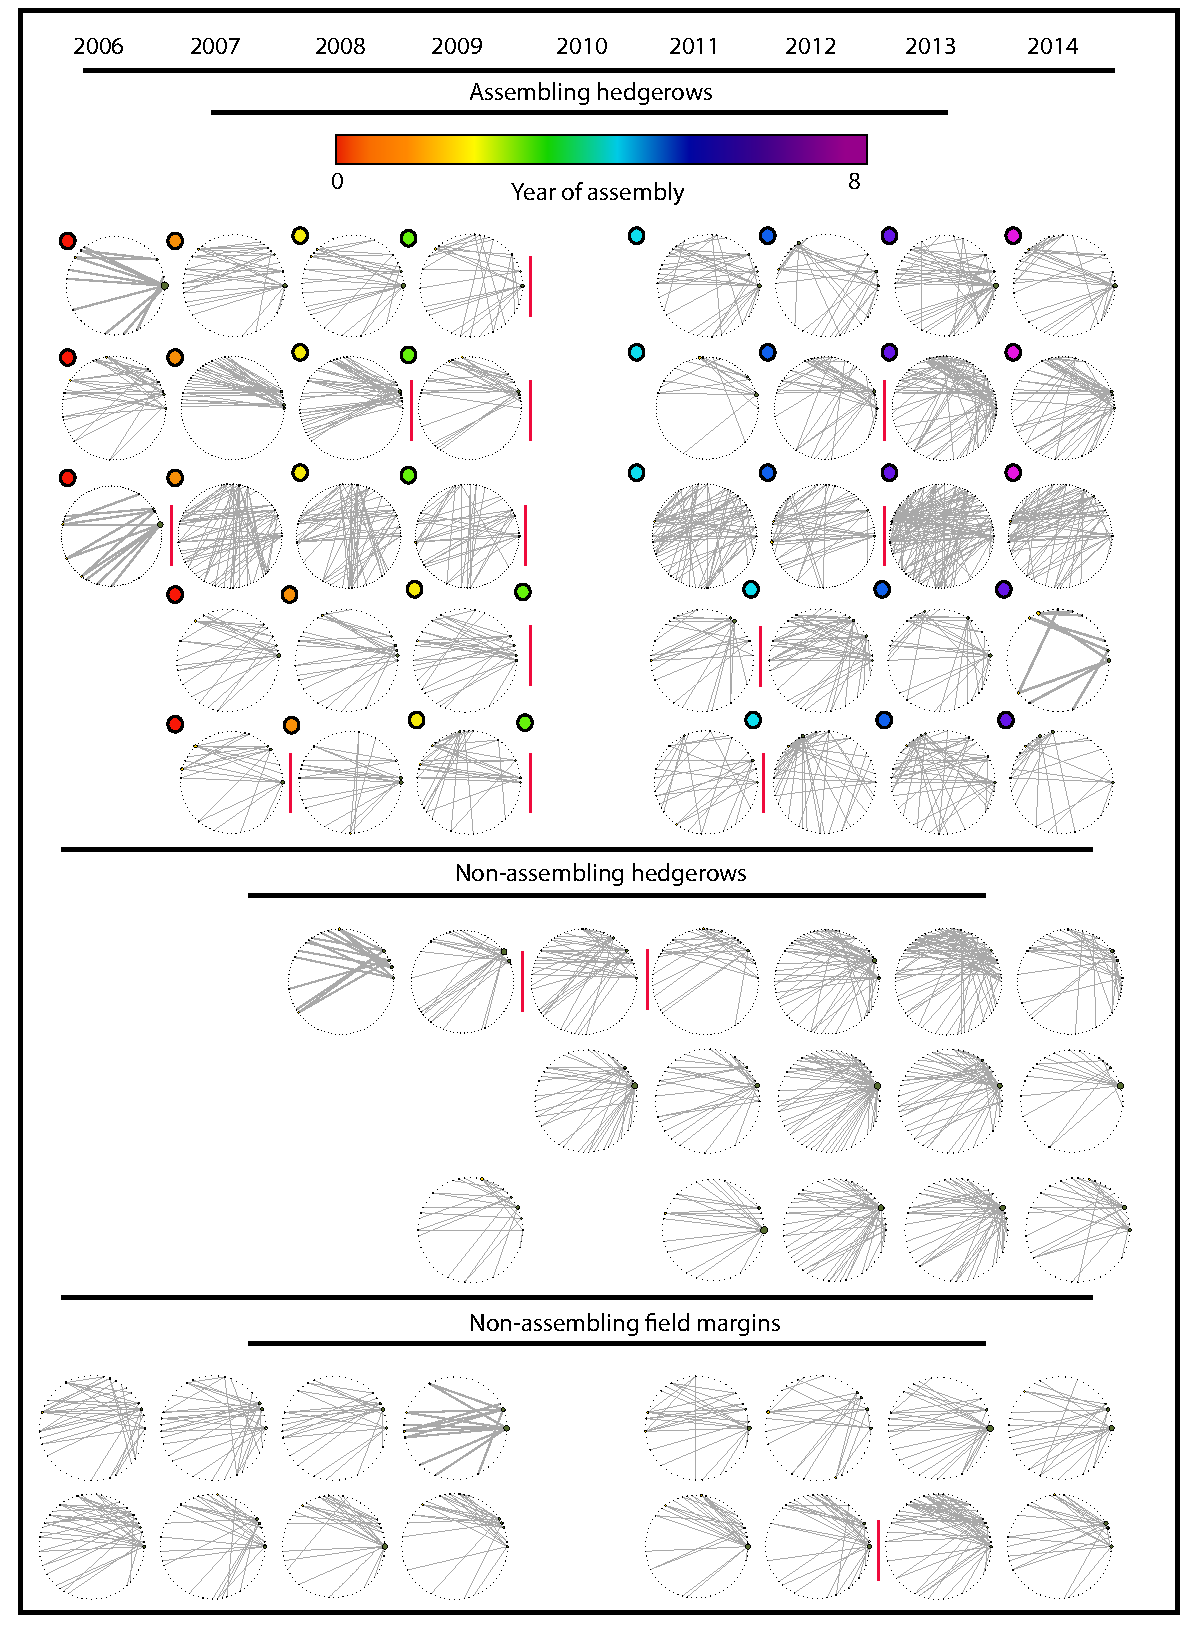
\includegraphics[width=.8\textwidth]{../analysis/changePoint/plotting/networks.pdf}
  \caption{XXX}
  \label{fig:changePoints}
\end{figure}
\clearpage

\subsubsection*{Characteristics of species that contribute to change
  points}

\begin{figure}
  \centering
  \includegraphics[width=.8\textwidth]{../analysis/variability/figures/cv/occ_degree.pdf}
  \caption{XXX}
  \label{fig:cv}
\end{figure}
\clearpage


% \subsubsection*{Characteristics of ``core'' and ``peripheral''
%   communities}

% \begin{figure}
%   \centering
%   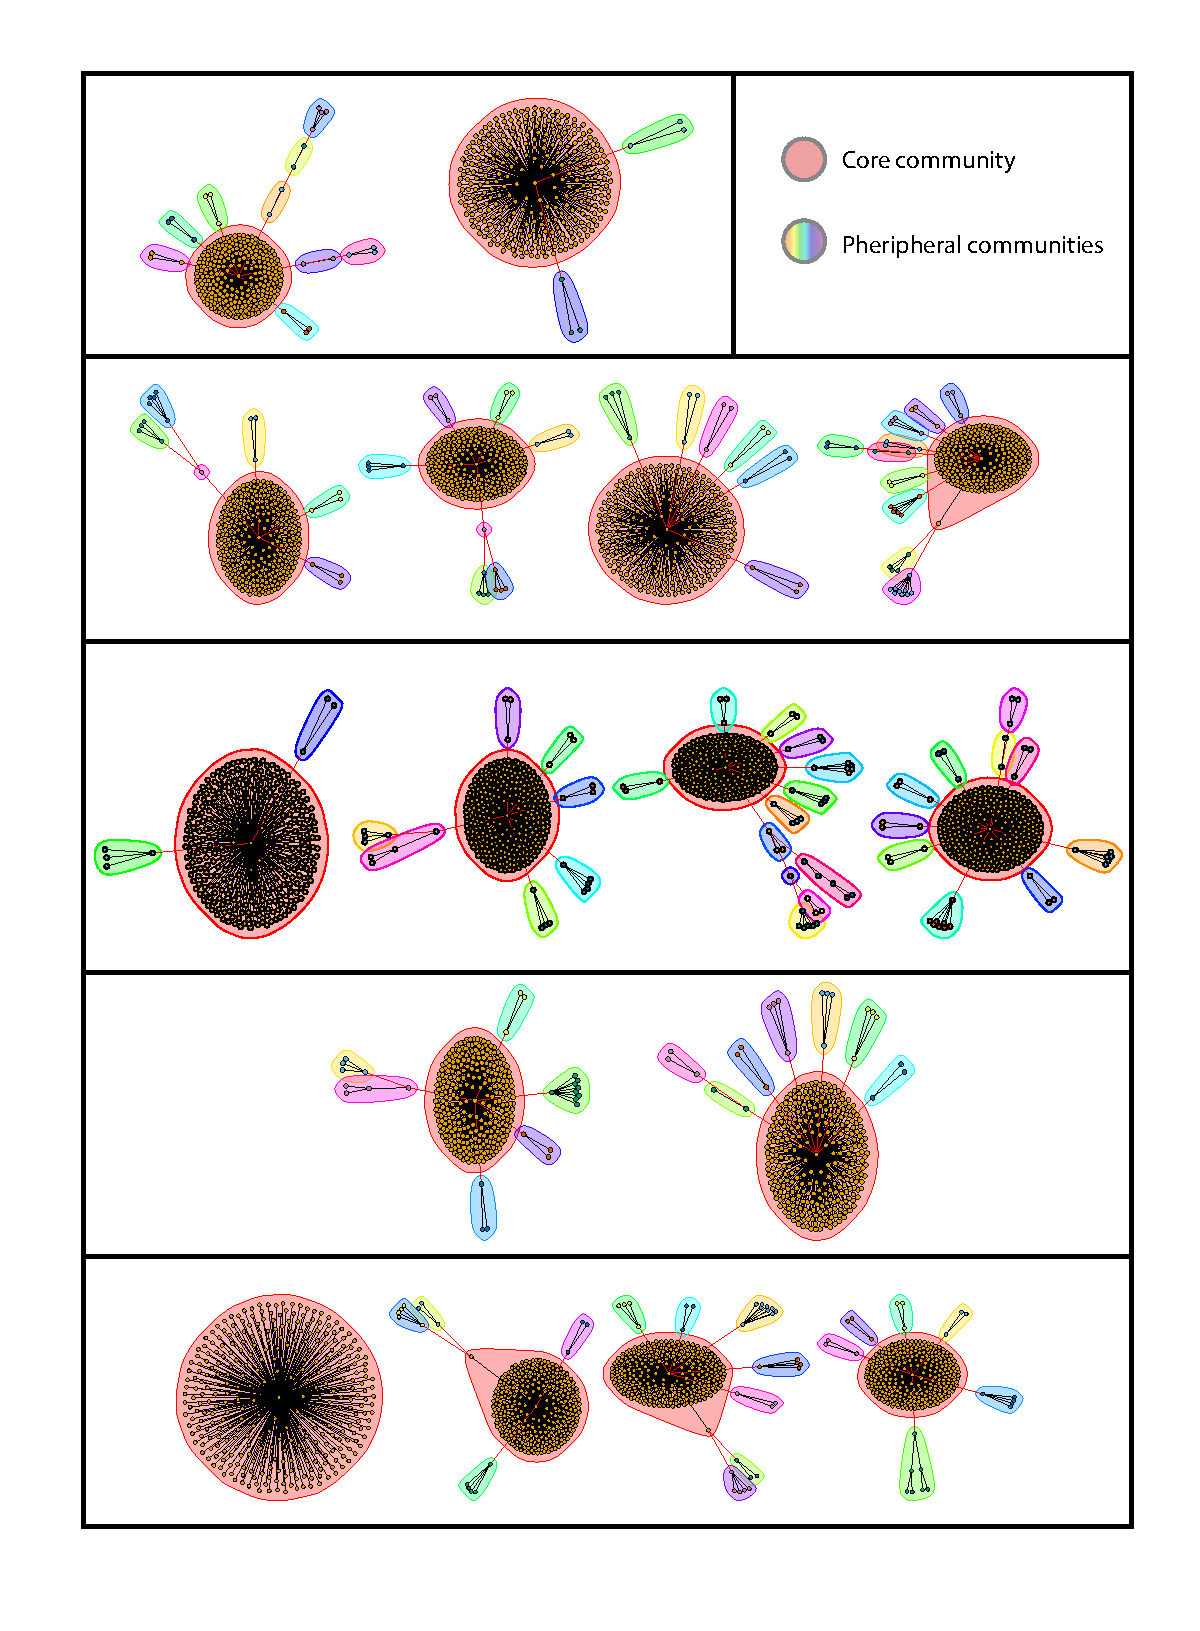
\includegraphics[width=.8\textwidth]{../analysis/changePoint/plotting/communities.pdf}
%   \caption{XXX}
%   \label{fig:communities}
% \end{figure}
% \clearpage

\begin{figure}
  \centering
  \includegraphics[width=.7\textwidth]{../analysis/changePoint/plotting/figures/pcoa/pcoa.pdf}
  \caption{XXX}
  \label{fig:pcoa}
\end{figure}
\clearpage

\subsection*{Network structure}

\begin{figure}
  \centering
  \includegraphics[width=.4\textwidth]{../analysis/networkLevel/figures/baci.pdf}
  \caption{XXX}
  \label{fig:baci}
\end{figure}
\clearpage

\subsection*{Network robustness}

%% no need for robustness figs bec not sig

\section*{Discussion}
\label{sec:discussion}

\section*{Acknowledgments}
\label{sec:acknowledge}

We would like to thank Leto Peel and Aaron Clauset for their
invaluable discussions and for help with the change point analysis.
We thank the growers and land owners that allowed us to work on their
property.  We also appreciate the identification assistance of expert
taxonomists Martin Hauser, Robbin Thorp and Jason Gibbs.  This work
was supported by funding from the Army Research Office
(W911NF-11-1-0361 to CK), the Natural Resources Conservation Service
(CIG-69-3A75-12-253, CIG-69-3A75-9-142, CIG-68-9104-6-101 and
WLF-69-7482-6-277 to The Xerces Society), the National Science
Foundation (DEB-0919128 to CK), The U.S.  Department of Agriculture
(USDA-NIFA 2012-51181-20105 to Michigan State University).  Funding
for LCP was provided by an NSF Graduate Research Fellowship and the
USDA NIFA Graduate Fellowship. FUNDING FOR MARILLIA.

\bibliographystyle{ecol_let}

\bibliography{refs}


\end{document}

%%% Local Variables:
%%% mode: latex
%%% TeX-PDF-mode: t
%%% End:
